\documentclass{lhcbnote}

\title{LHCb Performance and Regression}
%for more than one author %
\author{Emmanouil Kiagias}%,%
%with a different address %
% New Author{\address[NEWADD]{His address}%
%with the same address %
%Other Author{\addressmark[BGADD]}} %
%}%

\doctyp{Internal Note}
\dociss{1}
\docrev{0}
\docref{unknown}
\doccre{February 6, 2013}
\docmod{\today}
%\doccnf{You use this command only if you want a note %
% here: like presented at...}% 

\begin{document}

\maketitle

\begin{abstract}
Put your abstract here.
\end{abstract}

\begin{status}
\entry{Draft}{1}{February 6, 2013}{First version}
\end{status}

\tableofcontents

\listoffigures 
\listoftables

\section{Introduction}

What is { \bf LHCbPR }

\vspace{4 mm}

LHCb Performance and Regression(PR) is a service designed to record important measurements about releases of the 
LHCb application. Applications , such as Gauss, Brunel, Moore etc,  receive input in the form of configuration files 
and produce, as an output, various information.
LHCbPR is {\bf not} intended to actually run the jobs (maybe in the future as an extra feature), but instead to manage and track the bulk of information produced by them.
	
The LHCb Performance and Regression is a framework that allows LHCb software developer to push information for
a run of their code(job charactetistics, results, performance measures, files) to a central database, from which an analysis can be performed across
version, configs(platforms) etc.

\vspace{6 mm}

\noindent Why LHCbPR


\vspace{4 mm}

 In the past, in order for a user working group to run a  job, they had to execute a job for a specific application -using a configuration file-, 
gather the results and then run their own analysis on the produced sample. 
Finally, when such a process was complete, they needed to find a way to publish their results.
Often ending up with serving static documents such as HTML, CSV or e-mail.
	
LHCbPR was conceived as a tool to reliably organize the process of configuring and monitoring a job execution. 
The framework, solves the problem of gathering the results of a job execution, by providing the user a complete script that, when executed, 
can produce the desired output, according to a configuration file. This script, also includes a list of {\bf handlers} 
that collect the defined aspects of the job results and “push” them to the database in a uniformed way. 
	
By collecting the results in such an organized manner, it provides the solution to the second problem, mentioned above; 
the running of the analysis. Since, all the data are stored as objects in the database, 
the framework provides an abstract and easy way to deploy algorithms and functions which perform analysis on the saved data. 
	
Finally, LHCbPR handles the presentation of the collected data by providing a set of templates 
for the creation of web pages specific to each analysis and customized to the preferences of each user. 
 
\vspace{6 mm}

\noindent Users of LHCbPR


\vspace{4 mm}

The LHCbPR users can be divided into three categories: Administrators, Application developers and End users. 

The administrators group is responsible for the integrity of the collected data and the efficiency of the service. They maintain and support the system, 
making sure the application is functional and available to the end users.

Application developers are the users who actively design and develop modules for the framework, thus extending the functionality of the application.

Finally, the end users are the main body of the users of the service. They put the tools provided by the application developers to practical use and 
their job results are populating the database.

\section{Architecture}

\subsection{Django}

LHCbPR framework is written in python and the main body has been has been deployed with {\bf Django} . Django is an {\bf open source} web application framework, written also in Python.
 The application is hosted in a shared Apache web server with fcgi module. For more information about apache, fcgi and django can be found in their corresponding web pages.

\subsection{3TP - 3-Tiered Programming}

The LHCbPR follows the architectural model of three tiered programming. {\bf 3TP} provides a way to theoretically categorize the components 
of an application, providing abstract modularity. In essence the 3TP model is a client-server architecture which is composed of three 
layers. Namely,  the presentation tier, the functional process logic tier and the data storage tier. These tiers communicate with one another 
in a strictly defined way, which allows the developer to independently maintain each tier. In most practical applications of the model the presentation layer 
includes all forms of user interaction with the service. The process logic tier encompasses the whole of the application functionality, while the data storage 
tier handles the flow of the information from and to the data source (in most cases a database).

\vspace{4 mm}

The theoritical model mentioned above is practically implemented in LHCbPR(see Figure 1) and is explained in detail in the following sections. 

\begin{figure}[ht!]
\centering
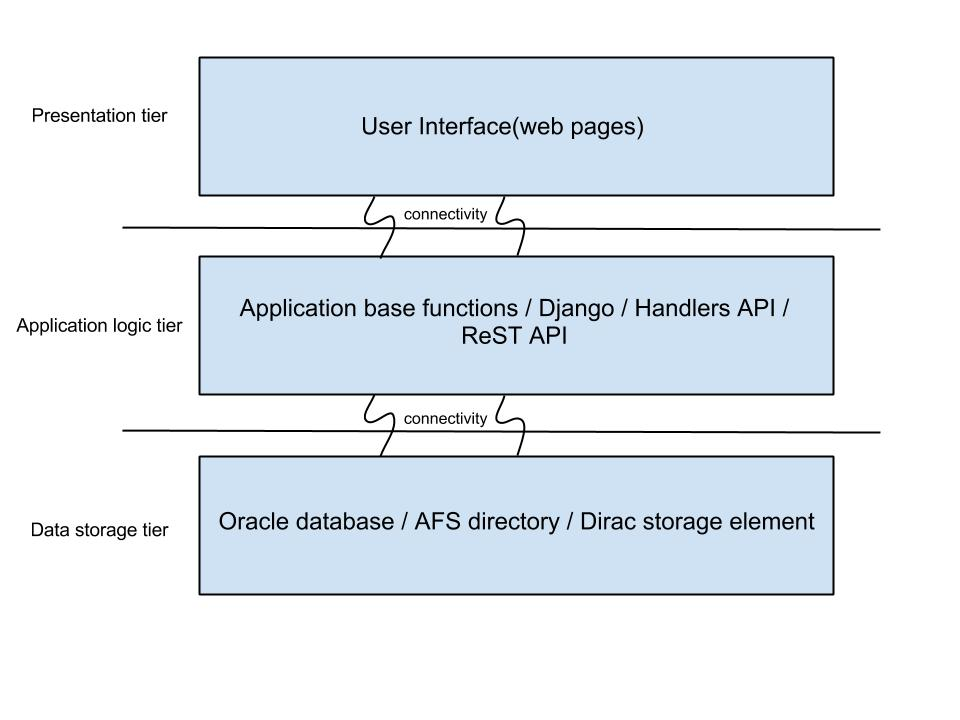
\includegraphics[width=170mm]{my3tp.jpg}
\caption{3TP implemented in LHCbPR}
\label{overflow}
\end{figure}

\subsubsection{Presentation layer in LHCbPR}

The presentation tier of LHCbPR is composed of a set of web pages that utilize a {\bf ReST} API, and the handlers' interface.

ReST comes from Representational State Transfer and provides an abstract way of stateless client-server communication. Django's capability of handling URLs, 
through the stateless HTTP Protocol, serves as a powerful tool to design and develop ReST Interfaces. LHCbPR's API functions range from generating and managing
unique identifiers(UID) for objects in database, to compiling scripts to run a simulation and collect their output.

Above the ReST API exists a set of web pages which are served to the end user by the django framework. These mainly consist of static HTML 
styling code and javascript/jquery functions that allow asynchronous communication with the ReST Interface. This web application provides an easy and 
visual way for the handling of the information stored in the database. 

The handler's interface is different to the ones mentioned above, in the sense that it provides a programmatical way to communicate with the service. 
That is, an application developer can use the handler library functions to strictly define the amount and type of data that will be collected from a job execution. 
Essentially the handler is an independent utility that can be called after any job execution to parse, group and collect specific information from the output.

\subsubsection{Application logic layer in LHCbPR}

The application logic tier a set of python modules that can be divided into two categories that each serve its own purpose; the base application logic and the 
database connectivity.

The base application logic is a group of functions which handles the incoming users' requests, sanitizes their input and generally tries to accomplish the application's 
objective. Also it provides an interface for application developers to specify the way they process the data that is stored in the database, by developing python 
modules for analysis. The development of such modules is abstracted from the specific implementation of the framework which makes the analysis process much 
simpler and more straightforward. 

The database connectivity is achieved by utilizing the models/views-function of the django framework. The representation of the content of the database as logical 
objects allows easy access and management of the stored data. Also it acts as a powerful mechanism for enforcing the db schema.


\subsubsection{Data storage layer in LHCbPR}

The third and last layer of LHCbPR is responsible for the data management of the whole service. It consists of three independent data sources. 

The first and most important is an Oracle database which is provided by the IT central Oracle service. It contains every bit of information about the jobs that 
have been executed, including the statistics and output information, apart from files. In case where whole files, produced from a job(e.g ROOT files), 
are needed to be saved then they are not handled from the database but from a filesystem.In the database is only saved a relative path, to a media directory, for each file .

The files mentioned are stored in an AFS shared directory for easy access and robust backup. 

Finally the last data source is another shared directory which is accessed through a DIRAC storage element and is used as a temporary caching space between the 
server and the data collected by the handlers. 


\section{Database}

In order to describe a job execution through the LHCbPR framework and generate a script which will run the defined-described job, {\bf job descriptions} are saved/handled as objects 
in the database. Also they are used to identify which data comes from which job execution. The database objects will be explained in details in the following subsections.

\vspace{4 mm}

Here is a summary of the database schema tables:

\vspace{4 mm}


\begin{tabular}{ | l |}
\hline
	
Jobattribute \\ \hline
	
JobDescription \\ \hline
	
JobHandler \\ \hline
	
JobResults \\ \hline
	
Options \\ \hline
	
Platform \\ \hline
	
Requested\_platform \\ \hline
	
ResultsString \\ \hline
	
ResultInt \\ \hline
	
ResultFloat \\ \hline
	
ResultFile \\ \hline

SetupProject \\ \hline
\end{tabular}



\subsection{Job description object}
The tables which constract a job description are the following:
\begin{itemize}
\item
JobDescription, Application, Options, SetupProject
\end{itemize}

The Application table contains two columns : appname(application) and appversion(application version).
This pair is unique for each application and ,as the name says, this table represents the application(eg Gauss, Brunel etc)
with a specific version(eg v42r0, v43r2p0 etc) and its data will be used to setup the environment to prepare a job execution for 
the corresponding application.

\vspace{4 mm}

The Options table represents the options which we will used to execute a job and it has two columns:
description and content. The description column is more or less a name(alias) to identify the options and the
content is the actual content of the options, which can be a path to an options file or a big string containing 
the actual raw options. Note that the pair description-content in the table must be unique, can not have the same 
description for two(or more) different contents or the same content for two(or more) different descriptions.

\vspace{4 mm}

The SetupProject table represents the extra arguments(optional) to the SetupProject command. Also this table has two
columns : description and content. The description is a name(alias) to identify the SetupProject extra arguments(eg --no-user-area)
and the content is the actual extra arguments. Note the pair description-content must me unique(same as the pair description-content of the
Options table)

\vspace{6 mm}

All the three previous tables constract a job description object. This is the information which is needed 
to properly configure and execute a job, this is the table (see Figure 2).

\begin{figure}[ht!]
\centering
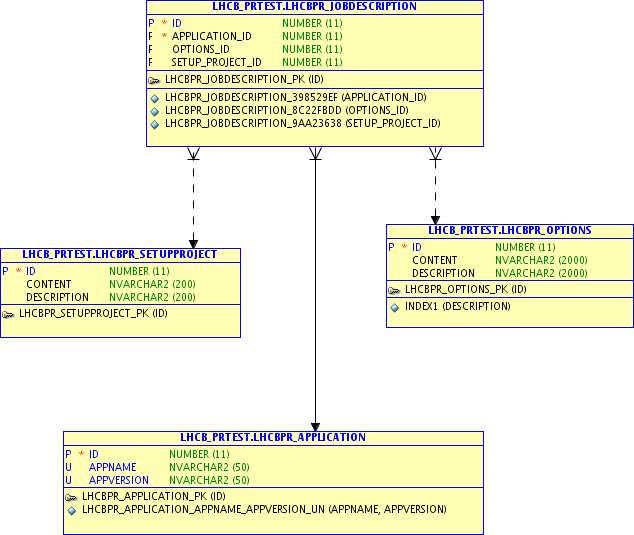
\includegraphics[width=170mm]{jobdescription.png}
\caption{Job description table summary}
\label{overflow}
\end{figure}


\subsection{Job}

Once there are saved job descriptions in the database they can be used to actually run jobs.
The Job table has the following columns: The jobDescription\_id, an id to specify which job description object 
was used to execute the job(application-version, options etc), the time when the job started and finished(time\_start and time\_end columns), 
the status of the job(finished, running etc), success(whether the job was successful or not). Also a job contains the platform(cmtconfig) 
and the host(machine) on which it was executed. Apart from the others, which are single columns, the platform and the host columns(and the 
jobDescription) are ids mapping to the corresponding tables Platform and Host. 

\vspace{4 mm}

The Platform table contains only one column containing a platform(cmtconfig).

\vspace{4 mm}

The Host table represents a machine(on which jobs are executed) and has the following columns:
hostname(name of the machine eg pclhcb10), cpu\_info and memory\_info for the machine.

\vspace{6 mm}

All the above constract a job object which represents a single job execution(see Figure 3)


\begin{figure}[ht!]
\centering
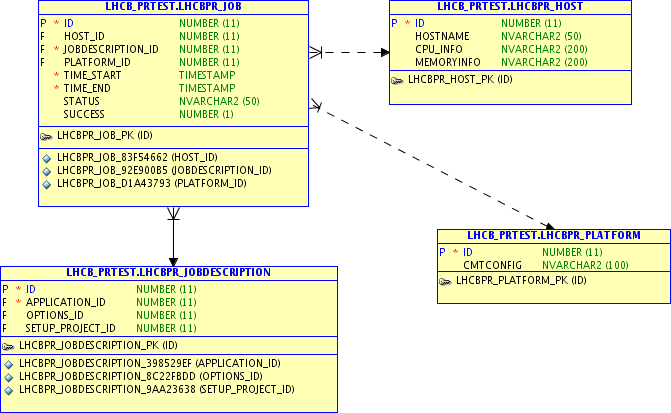
\includegraphics[width=170mm]{job.png}
\caption{Job table summary}
\label{overflow}
\end{figure}

\subsection{Job results}

Up to now we described how a job description and a job execution are represented in the database. 
Now we will see how job results are saved.
Each job execution produces various results such as log files, ROOT files(histograms), xml files etc.
A result can be a number(a float, an integer), a string or a whole file. Each result is considered 
to be a Job Attribute and it is saved in the JobAttribute table.

\vspace{4 mm}

The JobAttribute table represents,identifies a job result and has the following columns:
The name column which is the name the result will hold(eg totalCrossSection), the description(optional) 
column which is a description for the attribute, group column(optional) which specifies a group for 
the attribute(eg group: "Timing") and the type column which can be an Integer,String,Float or File. 

\vspace{4 mm}

The ResultInt,ResultString,ResultFloat,ResultFile tables "inherit" the JobAttribute table and just provide 
the data column for each job attribute. So the JobAttribute table works as the parent table and depending
on the type column it has a corresponding child table, example: if the type of a job attribute is "Integer"
then the it will have as its child a ResultInt.

To associate the previous tables, one with each other, and all together with the job table a middle
JobResults table is used which contains a JobAttribute\_id mapping to a JobAttribute object and each 
Result(ResultString etc) table contains an id mapping to a JobResults object(see Figure 4). 
Finally the JobResults table also holds a job\_id which maps to a specific job. 

\vspace{6 mm}

So for each job execution there are multiple JobResults instances containing the collected results.

\begin{figure}[ht!]
\centering
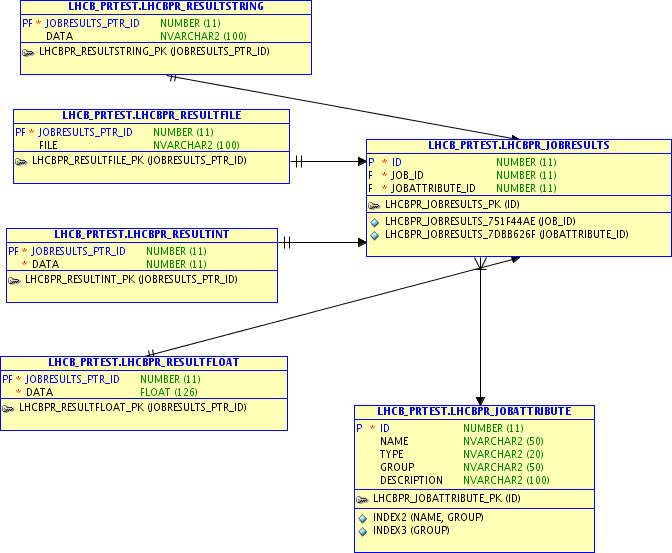
\includegraphics[width=170mm]{jobattribute.png}
\caption{Job attribute table summary}
\label{overflow}
\end{figure}


\subsection{Handlers}

Handlers are python modules which take as a parameter a directory and 
collect results out of it. Handlers can collect many kind of data
such as Numbers(Floats, Interger) ,Strings, even save a whole file. In order 
to associate handlers with jobDescriptions and job executions the following tables
are used: Handler, JobHandler, HandlerResult

\vspace{4 mm}

The Handler table represents a handler python module and contains two columns:
a name column which is the name of the python module and a description column 
which is a description(optional) about the handler. A handler can collect data from 
different jobDescriptions even from jobDescriptions with different applications
(example the TimingHandler works for all applications). A handler is associated with 
a jobDescription through the JobHandler table.

\vspace{4 mm}

The JobHandler table is used as a middle table(many to many relation) 
between the JobDescription and the  Handler tables.

\vspace{4 mm}

So for each JobDescription there are associated handlers which will collect data after a job 
execution. When a job is finished, the handlers(may be just one) collect data and produce a zip 
file with the results. In some cases though a handler can fail(either because of a user's mistake or because 
a job execution did not produce the results it should have produced), so we keep track of the handlers 
by using the HandlerResult table.

The HandlerResult table shows whether a handler was successful or not for a specific job execution, so
it contains a handlers\_id(to map a handler object), a job\_id which maps to a job execution and 
finally a column success to specify whether the handler was successful or not for this job.

\vspace{4 mm}

For the above tables see Figure 5.


\begin{figure}[ht!]
\centering
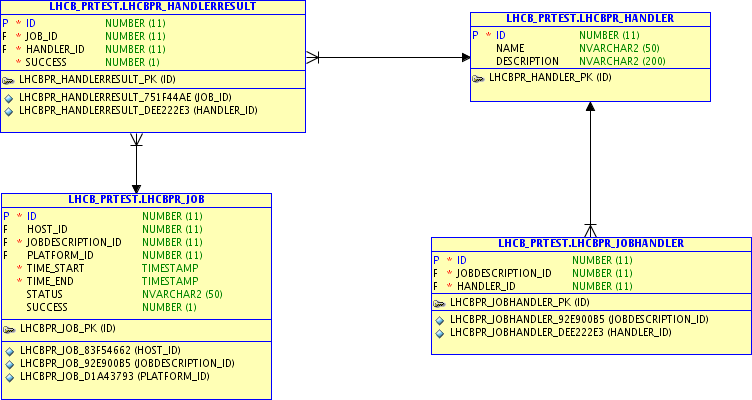
\includegraphics[width=170mm]{handler.png}
\caption{Handler table summary}
\label{overflow}
\end{figure}


\section{Implemented functionality}

Here follows a summary of the implemented functionality of the LHCbPR.

\subsection{Job Description Management}
\begin{itemize}
\item
\underline{Create new Job Description} 

A new job description can be created through a web interface by 
 cloning an existing job description(cloning means to create a new object based 
 on a preselected job description).

\item
\underline{Update Job Description}

A job description can be updated(change one or more attributes) through a web interface.
Warning: a job description can not be edited if there is at least one executed job saved in the database with this job description.

\item
\underline{Create Job Description from script} 

A job description can also be created from a script(by making an HTTP request with the desired attributes). 
In case the job description exists the function returns the existing job description id.

\item
\underline{Generate Job script}

A script which will execute a job using a selected job description. The script can either be created through a web 
interface(by clicking a button) or by making an HTTP request through a script.
\end{itemize}

\subsection{Job Handling}
\begin{itemize}
\item
\underline{Basic python handler interfaces}

An application developer can use the provided handler functions to strictly define the amount and type of data that will be collected from a job execution. 
\end{itemize}

\subsection{Analysis}
Here follows a summary of the already implemented analysis pages

\begin{itemize}
\item
\underline{Basic analysis}

In this analysis page the user can select a single quantity(a single attribute from the database eg EVENT\_LOOP) 
also select a job description(or part of it eg only specific options or platform)
and calculate the average value, standard deviation, generate a histogram for the corresponding selections. Up to 3 histograms can be generated at once 
and also be superimposed.

\item
\underline{Timing analysis} 

In this analysis the user can select a job description and generate a tree containg the average timing performance of the algorithms 
of all the available job runs for the selected job description.

\item
\underline{Histograms analysis} (available only for Gauss application) 

More or less the same as the basic analysis but in this case the user selects a histogram title(from the saved ROOT files) instead of a single quantity, 
and calculate the average histograms for all the available ROOT files. 
Also the histograms can be superimposed or divided(for the division there must be exactly 2 histograms , no more no less) 

\item
\underline{Trend analysis} (not fully completed yet) 

In this analysis the user can select a single quantity and perform an analysis across the versions of the application.
\end{itemize}

\subsubsection{Custom Analysis Framework}

Each analysis page is a module and all the above analysis pages are deployed using a small custom analysis framework. 
The development of such modules is abstracted from the specific implementation of the LHCbPR framework which makes the analysis development much 
simpler and more straightforward for the developers.

\subsection{Authentication}
All the LHCbPR's pages and services are protected by shibboleth, the user must provide a valid cern account in order to access the service.
Also there is the ability to restrict the access to only specific groups ,if necessary, in a desired service/services. 

There is also restricted access to the administrator panel. The admin panel can be accessed only from superusers which are defined inside the database through Django. 
For more info about superusers check the Django documentation

\subsection{Administration}
The LHCbPR also comes with a default administration panel provided from the django framework to manage database objects through a web interface. 
Also the LHCbPR provides a function to either delete a job by id or  hide a job(flag to hide bad data, these jobs will not be used in analysis pages). These 
functions can olny be accessed from the administrators. As mentioned in the above subsection only superusers can access the admin panel. 
For superusers check Django official documentation

\section{Analysis development}

The LHCbPR framework provides also the ability to develop new analysis modules and handlers. 
In this section will be descrided how to develop a new analysis module (a functional analysis web page) using a small custom framework 

\subsection{Getting started}

Below are described the steps you need to do in order to develop a new analysis module locally on your computer and test it. 

First get the latest version of the project from the LHCb git repository:

\vspace{2 mm}

{\bf git clone /afs/cern.ch/lhcb/software/GIT/LHCbPR.git}

\vspace{2 mm}

Then run the script :

\vspace{2 mm}


{\bf LHCbPR/devel/getdjango} (version of django is set, hardcoded, inside the script)

\vspace{2 mm}

This will download the Django source and place inside the LHCbPR/devel directory . 
The LHCbPR is deployed with Django framework so you need a copy of it in order to 
run the service locally.

After that you need tou setup the enviroment in order to use the cx\_Oracle module from afs:

{\bf Note}: the script works on {\bf bash} not in tcsh/csh etc.
\vspace{2 mm}

{\bf source LHCbPR/devel/setuptools}

\vspace{2 mm}

The LHCbPR uses an oracle database
so it needs the cx\_Oracle to establish a connection with it(in case you have not executed the getdjango script the setuptools script will invoke it to download the django for you).

{\bf Attention}. One more step to finish the setup. You must provide a {\bf myconf.py}
file in {\bf LHCbPR/django\_apps/} directory in this format:

\begin{verbatim}
dbname = 'name_of_the_database'
dbuser = 'username_for_the_database'
dbpass = 'database_password'

key = 'key_django_needs'

#ATTENTION
# LOCAL must true in order to run the project locally
LOCAL = True

#also debug true is needed to get the django's debug page
#in case an error happens
DEBUG = True

#root url for the local development needs to be /
ROOT_URL = '/'
\end{verbatim}

{\bf Note}: Ask the administrator to give you the needed information (dbname,dbpass etc). If you have access 
to {\$LHCBSOFT/webapps/LHCbPR/LHCbPR/} copy the {\bf myconf.py} file from there (remember to use the testing or developing database not the production one when 
deploying locally). In case you copy the file from \$LHCBSOFT do not forget to change the settings as shown above (eg  LOCAL variable to LOCAL = True, ROOT\_URL = '/' etc). 

\vspace{2 mm}

And once you have the myconf.py file {\bf everything's ready} in order to start running your local copy (you must keep the runserver command running to make your local LHCbPR work):

\vspace{2 mm}

{\bf LHCbPR/django\_apps/manage.py runserver}

\vspace{2 mm}

Do not forget to run the {\bf source LHCbPR/devel/setuptools} everytime you change {\bf shell}(eg: work the project in a new terminal) 
in order to setup the enviroment with the needed tools(without this script the runserver command will crash).

\subsection{Writing a new analysis module}

{\bf Note}: Before you continue it is suggested that you take a look about {\bf django templates} (in case you are not familiar), more info can be found {\bf https://docs.djangoproject.com/en/dev/topics/templates/}

\subsubsection{Initialization}

Once you have downloaded a local copy of LHCbPR project from git and set up the enviroment you are ready to start deploying your new analysis module.
First create a {\bf new folder} with the name of your new module under to {\bf LHCbPR/django\_apps/analysis} directory. Let's assume your new analysis module will be called {\bf hello\_analysis} , then create a folder :

\vspace{2 mm}

{\bf mkdir LHCbPR/django\_apps/analysis/hello\_analysis}

\vspace{2 mm}

Then create an \_\_init\_\_.py under your new created directory(your analysis code will reside in there) :

\vspace{2 mm}

{\bf vim LHCbPR/django\_apps/analysis/hello\_analysis/\_\_init\_\_.py}

\vspace{4 mm}

Each analysis module must have two basic {\bf templates} in the templates directory:
 \begin{itemize}
\item
{\bf render.html}
\item
{\bf analyse.html}
\end{itemize}

The {\bf render.html} is the one that will be used to diplay the contents of your analysis page
and the {\bf analyse.html} is the template that will be used to diplay the actual analysis results(this template is loaded inside the render.html automatically), 
create them in the templates' directory under a directory having the name of the analysis(same we did with the module) :

\vspace{2 mm}

{\bf mkdir LHCbPR/django\_apps/templates/hello\_analysis}

\vspace{2 mm}

{\bf vim LHCbPR LHCbPR/django\_apps/templates/hello\_analysis/render.html    (2)}

\vspace{2 mm}


{\bf vim LHCbPR LHCbPR/django\_apps/templates/hello\_analysis/analyse.html} (this is not mandatory for the beggining)
 \vspace{2 mm}

The render.html template has to follow a skeleton structure. The skeleton is available at:

\vspace{2 mm}

{\bf vim LHCbPR/django\_apps/templates/analysis/skeleton\_analysis.html     (1)}

Note, to copy the skeleton to you render.html use: {\bf cp (1) $\rightarrow$ (2)}	

\vspace{2 mm}

The above skeleton can be extended or use as is. Instructions on how to use or extend the skeleton are in the file itself. 

\vspace{2 mm}

The {\bf docstring} of the \_\_init\_\_.py file(your module's docstring) will automatically be used as {\bf helptext}(help div in the template) in your new analysis page.
In case you dont provide a docstring then the helptext will be "This module is not documented yet". In case you want to hardcode the helptext inside your render.html template
then follow the instructions in the skeleton\_analysis.html.

The {\bf title} of your analysis page will automatically be the selected application followed by the name of your module, so in our case of hello\_analysis module and GAUSS application,
the title of the page will be "GAUSS hello\_analysis analysis". In case you want to {\bf override} the default generated title, just provide a variable by the name title in your \_\_init\_\_.py file:

\vspace{2 mm}

\begin{verbatim}
#this will be now your page title
title = "This is my page title"
\end{verbatim}

\vspace{2 mm}

Edit the \_\_init\_\_.py file in your analysis directory and add the 3 following needed methods :

\begin{itemize}
\item
{\bf def isAvailableFor(app\_name):}
\item
{\bf def render(**kwargs): }
\item
{\bf def analyse(**kwargs):}
\end{itemize}

\subsubsection{isAvailableFor(app\_name):}

Once you have created your analysis module(folder etc), as mentioned above, it's time to specify for which applications the analysis is available for.
For example the "histograms" analysis is available only for the GAUSS application so the \_\_init\_\_.py file of the histograms module has the following method:

\begin{verbatim}
def isAvailableFor(app_name):
    if app_name in ['GAUSS']:
        return True
    
    return False
\end{verbatim}

Everytime you select an application from the analyse page, the LHCbPR "walks" in the analysis' module directory and calls in a sequence 
the isAvailableFor(app\_name) method from every  module. If the method returns "True" then the analysis will automatically appear as 
button in the rendered page, else if it's "False"  it wont appear. So in case you want to make your analysis available for all applications you can just do:

\begin{verbatim}
def isAvailableFor(app_name):
    return True
\end{verbatim}

In that way, no matter what the app\_name variable contains the method will always return True so it will appear to all applications

\subsubsection{render(**kwargs)}

The {\bf def render(**kwargs) } function returns the {\bf render.html} to the web browser, which resides in the templates/hello\_analysis/directory,
along with a dictionary with all the variables you want to use in your render.html template, 
for example:

\vspace{2 mm}

\begin{verbatim}
def render(**kwargs):
    myvariable = "test_string"

    return { 'myvarialbe' : myvariable }
\end{verbatim}

\vspace{2 mm}

This will return the render.html template along with the myvariable which you can access it in the template with: \{\{ myvariable \}\}. 
Before you continue please make sure you have checked how a render.html file must be in {\bf LHCbPR/django apps/templates/analysis/skeleton\_analysis.html}.

As it is mentioned in the skeleton\_analysis.html your render.html inherits the Versions, Options, Platforms, Hosts selections menu.
By default the LHCbPR returns the Versions, Options, Platforms, Hosts objects for the successful jobs of the corresponding application.

\vspace{2 mm}

{\bf Note}, for example in the {\bf timing analysis} we need, not only the objects for the successful jobs but also we need the objects who also have jobAttributes with some specific groups, so in that
case we override the default values which LHCbPR returns.

So if you want to return different objects then you can {\bf override the default values} by providing 'options', 'versions', 'platforms', 'hosts' in your returned dictionary. Here follows an example of how we override the default values in the timing analysis:



\begin{verbatim}
#missing code here ...
#...
from lhcbPR.models import Host, Platform, Application, Options

def render(**kwargs):
    #some missing code here
    #....
    app_name = kwargs['app_name']

    #some missing code here, for full version,
    #you can check the LHCbPR/django_apps/analysis/timing/__init__.py
    #....
    options = Options.objects.filter(jobdescriptions__jobs__success=True,
        jobdescriptions__application__appName=app_name,
        jobdescriptions__jobs__jobresults__jobAttribute__group='TimingTree').distinct().order_by('description')
        
    versions = ...
    
    platforms = ...
     
    hosts = ...
    
    dataDict = {
                'platforms' : platforms,
                'hosts' : hosts,
                'options' : options,
                'versions' : versions,
               }
      
    return dataDict
\end{verbatim} 

In that example you can see that we override the options,platforms etc by providing our own objects. That way
the template will use these objects instead of the default ones. 

{\bf Important}: if you are not familiar with the above overriding example and you wish to override the default values for your analysis then it is suggested you take a look in the {\bf django models} at :
 {\bf https://docs.djangoproject.com/en/dev/topics/db/models/}

\vspace{4 mm}
In the {\bf render(**kwargs)} you can access the following data:

\begin{verbatim}
# you can take the application from the url(such GAUSS, BRUNEL etc)
app_name = kwargs['app_name']

#the data which request contains,
# same as doing ,in case of POST request: requestData = request.POST
requestData = kwargs['requestData']

#and finally, in case you need to have access to the full request object
myrequest = kwargs['request']
\end{verbatim}

\subsubsection{analyse(**kwargs)}

This function will automatically  be called when you press the "Retreive results" button from your analysis page 
and here you need to implement what shown as results of the analysis.  
Same as the render function you can access the same data from the kwargs as shown exactly above(app\_name, requestData and request). 
Once you click the "Retreive results" button the page will automatically make an {\bf ajax request} to your analyse(**kwargs) sending the 
selected Versions, Options, Platforms, Hosts(comma separated ids) from the selection menu along with the data of your other custom elements
Let's assume that you have these two elements in your render.html template:

\begin{verbatim}
<input id="firstName" type="text" value="Emmanouil">
<input id="lastName" type="text" value="Kiagias">

<input id="myradio" name="myradiobutton" type="radio" checked="checked">
\end{verbatim}

The page will put the id and the value of your elements in the request dictionary along with the selected Versions, Options..etc object, so in this case the request dictionary will like this:

\begin{verbatim}
{
  'options' : 1,5,7, # comma separated primary keys of the selected options 
  'versions' : 3,5 , 
  'platforms' : 45,7,9,
  'hosts' :78,
  'firstName' : 'Emmanouil',
  'lastName' : 'Kiagias',
  'myradio' : True
} 
\end{verbatim} 

You can access these data from the kargs['requestData'] dictionary. Then in your analyse(**kwargs) function you can use these data to make queries to the database(check: from django.db import connection)
and any other calculation you need to produce your analysis results and just return a dictionary with your data. The analyse function will load the analyse.html template along with your data in the render.html template.
So you can visualize your results with javascript,jquery etc, or any other web tools in your analyse.html template and they will be loaded in your analysis when you press the "Retreive results button".

\subsubsection{Retrieving results from database}

Once you have the input data you need from your analysis page you can use it and query the database. Django provides various ways to query information from your database. For example way is through the {\bf django models} (django model API, which in our case is not the preferred way unless your query is very simple, more info: {\bf https://docs.djangoproject.com/en/dev/topics/db/queries/}) or another way is through the {\bf python cursor}.

In most of our cases we will need to write an sql query and execute it through {\bf the cursor}, then fetch the results from the cursor. Here follows an example of how the cursor works:

\begin{verbatim}
from django.db import connection
#
#...
#

def analyse(**kwargs):
    requestData = kwargs['requestData']
    #let's assume your and attribute id in your requestData
    atr_id = requestData['atr']
    
    #establish connection with db, get the cursor
    cursor = connection.cursor()
    
    #then execute your query(here is an example, not real functional)
    cursor.execute('SELECT * FROM lhcbpr_jobattribute WHERE id='+atr_id)
    
    #then get you resutls, either fetch them all
    #myresults = cursor.fetchall() #here it returns a list with the selected rows
    
    #or loop over one by one, preferred if you want to handle 
    #each selected result independently 
	
	#get one result from the cursor
    result = cursor.fetchone()
    
	myList = []    
    
    #loop while there are no results left
    while not result == None:
        #do stuff here with the result
		#...
		#add my result in myList
		myList.append(result)        
        
        #read the next result
        result = cursor.fetchone()
    
    #once out of the loop, do stuff with my myList
    #...
    #then return my results to be displayed through my analyse template
    
    return { 'myresultsList' : myList } 
    
\end{verbatim}

{\bf IMPORTANT}: in case you are not familiar with the {\bf python cursor} you should check how things work before you start writing your analysis and quering the database, a quick full quide can be found here: 
{\bf https://docs.djangoproject.com/en/dev/topics/db/sql/}.

\vspace{2 mm}

Also in order to get a better understanding how the LHCbPR's database is structured and how to query information you can read the database section of the documentation and/or also take a look into the existing analysis modules (basic, timing) and take ideas out of them.

\subsubsection{Using different templates}

The default behavior of the functions is: the render(**kwargs) function uses the render.html with the data of the dictionary you return 
and the analyse(**kwargs) function uses the analyses.html with the data of the dictionary you return. You can {\bf override} the default by specifying
a {\bf template key} in the returned dictionary with the different template you want to use. For example in the {\bf timing analysis} we have 3 different ways of visualizing the data:
TreeGrid, TreeMap, singleLevel so we have different analyse templates. So in case we want to use the analyseTreeMap.html(a different template we created in the templates/timing/  directory)  instead
of the default analyse.html template  in the analyse(**kwargs) function we do :

\begin{verbatim}
return {
         #....            
         #here reside the data we need in our template
         #and here we override the template to be used:
         'template' : 'analysis/timing/analyseTreeMap.html'
       }
\end{verbatim}

Also there are some templates for general use  in the templates/analysis directory like the error.html, so in case an error occurs with your data of with the database inside the analyse(**kwargs) or the render(**kwargs) function
then you can do:

\begin{verbatim}
if Error:
  return {
           'template' : 'analysis/error.html'
           'errorMessage' : 'My errorMessage accessed by {{ errorMessage }}'
         } 
\end{verbatim}

This way you are able to create as many templates as your needs to diplay different messages, visualize in different ways your analysis results 
by overriding the template variable in the returned dictionary.

\subsubsection{Bookmarking, trigger results, errorChecking}

The template ,which your render.html, inherits provides {\bf automatic bookmarking} with the following functions:

\vspace{2 mm}
\begin{itemize}
\item
prefillAll();
\item
prefill(); //per object
\end{itemize}

The prefillAll() will take the values from the url(GET request data) and will prefill the elements by id(keys of GET dictionary), or the prefill()
will just perform the previous action for a specific values( also check the {\bf trigger()} in the example code).
So if you want to enable {\bf bookmarking } in your render.html you can have something like this:

\begin{verbatim}
$(document).ready(function() {
 /* in case you want to prefill a single element you can 
  * you can use this jquery function .prefill() :
  * $("#my_element_id").prefill();
  */
  //or else you can just call prefillAll();  
  prefillAll(); 
  /* this method will take the values from the url(GET request data)
   * and will prefill all the available elements with the specified values
  */
 /* also if you want to automatic retreive the results in the 
  * bookmarking url call trigger in your code :
  trigger();
 /* this will "click" the retreive results if the url contains trigger=true
});
\end{verbatim}

Finally if you want to make {\bf errorchecking} to your elements' values before the ajax request from the "Retreive results" button you
can define a function called: {\bf checkRequestData(requestData)} in your script block in the render . Let's assume that in your analysis
page you want to always have at least two options selected before you press the button to retreive the results, in case the user doesn't
select less than two options then an error message should be printed with the problematic field and the reason of the error, example code :

\begin{verbatim}
function checkRequestData(requestData){
//the requestData dictionary contains the data 
//that will be sent to the analyse(**kwargs) in the format
//we previously mentioned
  //initial empty error object
  var errors = {}
 
  var myoptions = requestData["options"].split(",");
  if (myoptions.length < 2)
    errors["options"] = "At least two options must selected!";

 return errors;
}
\end{verbatim}

The {\bf checkRequestData(requestData)} method will automatically be called , before the ajax request to the corresponding analyse(**kwargs) function of the analysis module, 
 passing the request data to it. If the returned errors' object is empty then the ajax request will be performed and the analyse.html template will be loaded to the page, if the 
errors object is not empty then a dialog will pop up printing the problematic fields (keys of the errors' object) along with the reason (values of the keys) and the ajax request 
won't be performed. 

In our example we create an empty error object.
If the user doesn't select at least two options we add an entry to the object error['options'] , as key we give a name for the problematic field(can be any word not necessarily the element id) and as
value we give the reason.

\subsubsection{Adding extra functions to the analysis}

Let take the case you need from your render.html to perform an extra asynchronous request with your analysis module before you retreive the results,
(for example the attributes filtering by group in the basic analysis). 

Let say that you want an extra function to hello\_analysis module called getMyStuff, then you have to define a method in your module like:

\begin{verbatim}
def getMyStuff(**kwargs):
  #the kwargs here contain again the request and requestDat
  # as the analyse(**kwargs) function
  #your function's code from here:
\end{verbatim}

To access your new extra method through ajax you must make the request to the following url:

\begin{verbatim}
url = "{{ ROOT_URL }}analyse/hello_analysis/functions/getMyStuff/"+appName;
\end{verbatim}
The {\bf ROOT\_URL} is returned to all LHCbPR templates so just use it the way it is, the same with the {\bf appName} variable.
So here follows the format of the url to access your extra function(change only the bold words) :

\vspace{2 mm}

url = "\{\{ ROOT\_URL \}\}analyse/{\bf name\_of\_your\_module}/functions/{\bf extra\_function\_name}/"+appName;

\subsubsection{Logging analysis}

For logging in your analysis module you can use the django loggers (python logging module), here follows an example:

\begin{verbatim}
import logging

#important get the analysis_logger
logger = logging.getLogger('analysis_logger')

def render(**kwargs):
    logger.info('I am inside the render function!')
    #
    #...
    #
\end{verbatim}

Using the {\bf analysis\_logger} from django (check the loggers in the LHCbPR's settings.py file) will save the logs in the LHCbPR's logs directory under the file: {\bf LHCbPR/django\_apps/static/logs/analysis.log}.

For more info on django logging:  {\bf https://docs.djangoproject.com/en/dev/topics/logging/}

\subsubsection{Accessing ROOT through subprocess in LHCbPR}

LHCbPR production release is deployed on a shared apache server. In the machine where the service is hosted ROOT is not installed thus we can not (and do not want to) access ROOT modules through pyROOT straight from the LHCbPR django process. For that reason when we want to use ROOT in LHCbPR we open a \textbf{subprocess} (from the main process) in which we communicate with a function (a custom function we write ourselves) which can import and use  pyROOT. 

The main process communicates, exchange messages/data, with the subprocess (we can also call it child process) through a \textbf{pipe}. In order to make the communication easier we wrapped the \textbf{pipe} inside a class called \textbf{subService}. The \textbf{subService} class can be found the following python file:

vim \textbf{LHCbPR/django\_apps/tools/viewTools.py}

\vspace{2 mm}

The subService class provides the following \textbf{methods}:
\begin{itemize}
\item
\textbf{connect}: opens a subprocess calling the \textbf{ROOT\_service.py} (will be explained later)
\item
\textbf{send}: sends data (any data, objects etc) to the subprocess (ROOT\_service.py)
\item
\textbf{recv}: receive data from the subprocess
\item
\textbf{finish}: does nothing, was kept for legacy reasons (compatibility with another subService class) 
\end{itemize}

The subService class opens a subprocess when the user calls the \textbf{connect} function. The subpService calls the ROOT\_service.py in a subprocess passing the needed environment so the ROOT\_service.py can access pyROOT, this python file can be found:

vim \textbf{LHCbPR/django\_apps/tools/ROOT\_service.py}

\vspace {2 mm}

So the user can access any python function from the \textbf{ROOT\_service.py} file through the subService class. 

Ok now let's assume that from your analysis module you want to access pyROOT (eg in order to handle a ROOT file which contains histograms). First you need to write your \textbf{python function} which will handle your data using ROOT and place it inside the \textbf{ROOT\_service.py} (check other function inside ROOT\_service like basic\_service etc). Once you have your function inside the ROOT\_service.py you can access it through the subService class from your analysis module. Your main process (analysis module) will communicate with the ROOT\_service through the \textbf{send} and \textbf{recv}(receive) methods of the subService class. Here follows an example showing how to write a "remote" function and access it through the subService class.

\vspace {2 mm}
Let's assume that your remote function (inside the subprocess) will take two numbers, will calculate their sum and return it back to the father proccess. Here is the function:

\begin{verbatim}
#your function must take a remoteService object (subService instance)
#in order to communicate with the father process
def calculate_sum(remoteService):
    #receive the first number from the father process
    first_number = remoteService.recv()
    
    #get the second number
    second_number = remoteService.recv()
    
    #calculate the sum
    sum = first_number + second_number
    
    #send the answer back to the father process
    remoteService.send(sum)
    
\end{verbatim}

Place the above function inside the ROOT\_service.py then \textbf{very important} and \textbf{mandatory} place an entry inside the functionList dictionary (a dictionary inside the ROOT\_service.py file) passing as key the name of the function and as value the function itself(like a pointer to the function), shown as below:

\begin{verbatim}
functionList = {
    'histograms_service' : histograms_service,
    'basic_service' : basic_service
    #any other function may exist here...
    #here add your new added function passing the name
    #of the function as key and value pass the function
    'calculate_sum' : calculate_sum
                }
\end{verbatim}

Once you have done the above you ready to access your "remote" function from your analysis module, here follows an example:

\begin{verbatim}
#import the subService class
from tools.viewTools import subService

#
#...
#

def analyse(**kwargs):
    #
    #...
    #

    #define the two numbers to calculate their sum    
    number1 = 10
    number2 = 20
    
    remoteservice = service()
    #open the subprocess
    #in case any error occurs return an error, example
    if not remoteservice.connect():
        #logger.error('Could not connect to remote service')
        return { 'errorMessage' : 'Connection with remote service failed!', 
                'template' : 'analysis/error.html' }
    
    #IMPORTANT    
    #once you call connect
    #define which method(function) from the subService you want to use
    #pass to the send method the name of your function as string  
    remoteservice.send('calculate_sum')   
    
    #once you call your method you can start communicating with it
    #send the two numbers
    remoteservice.send(number1)
    remoteservice.send(number2)
    
    #then receive the sum the child process (subprocess)
    my_number_sum = remoteservice.recv()
    
    #...
    #
\end{verbatim}

That way you can write methods which can have \textbf{access to pyROOT} (remember the ROOT\_service.py can import ROOT). The above way to access ROOT in LHCbPR may seem a little inconvenient but it is the only way for the moment. In the future(soon enough) when the \textbf{root.js}, accessing ROOT functions will become much more easier without the need to run ROOT on a local machine or communicating with other processes (as we do now).

\section{Handler development}

In this section we will show how to write and test a new handler to collect your data.

\subsection{Getting started}

First get the latest {\bf LHCbPRHandlers} project from LHCb GIT repository:

\vspace{2 mm}

{\bf git clone /afs/cern.ch/lhcb/software/GIT/LHCbPRHandlers.git}

\vspace{2 mm}

Then make sure you are using at least {\bf python2.6} to write and test your handler python module.
Once you have python2.6 and a local copy of the LHCbPRHandlers project you ready to start.

\subsection{How to write handler}

Each handler is python module which {\bf extends} the {\bf BaseHandler}(it resides in the {\bf LHCbPRHandler/handlers} directory)
and works as a parser which collect data. The only difference from any usual parser if the way it saves the attributes.

\vspace{2 mm}

The {\bf BaseHandler} class provides the following methods:
\begin{itemize}
\item			
saveInt
\item
saveFloat
\item
saveString
\item
saveFile
\end{itemize}

Each of the above methods take 4 arguments
\begin{itemize}
\item
{\bf name} : the name of the attribute you save( example : 'cpu\_execute\_time')  
\item
{\bf data} : the data/value your attribute has (example : 12.45)
\item
{\bf description}(optional) : any description you want to add for the attribute (example : 'this number represents...')
\item
{\bf group}(optional) : the group(if any) in which the attribute you save belongs(example : 'Timing')
\end{itemize}

Let take for example the following case:

\begin{verbatim}
execution_time = 12.45  
#If you want to save the number above you can save it like:

# remember the 4 arguments: name, data, description, group
self.saveFloat('execution_time', 12.45,'the total execution time', 'timing results')
					
#or just save it without description/group, just its name and its value/data:
self.saveFloat('execution_time', 12.45)					
\end{verbatim}

{\bf Remember} to use the right method for the corresponding {\bf type}, if you want to save  a string use the saveString function 
if you want to save an Integer use saveInt etc

You can also save {\bf files}(eg .root files) by calling the {\bf saveFile} function giving a 'name' for your file attribute 
and a 'filename' which must be the actual path to the file you want to save. For example:

\begin{verbatim}
#lets say that you have a file: my_results_file = '/afs/cern.ch/path_to/my_file'
##				attribute name 			path to file
self.saveFile('my_results_file' , '/afs/cern.ch/.../path/my_file' )
					
#also you can add a group and/or a description(like the explained above)
\end{verbatim}

The handler python file must have the same {\bf name} as the {\bf handler class},
For example if your handler class is called 'TimingHandler' then the python file must have the name 'TimingHandler.py'
		
Second you must have an \_\_init\_\_  where you call super(self.\_\_class\_\_, self).\_\_init\_\_() (as shown in the example below)
		
At last you must override the method collectResults(self,directory).
When a handler is invoked after a job execution , the script which invokes the handler passes to it 
a directory which contains the job results. So any file your handler needs must be found it in the given directory (the directory argument of collectResults function). In other words the directory argument will provide the path of the directory where the output of the job reside. You can there access the files by their names. Usually the \textbf{stdout} of the job is saved in a file under the name \textbf{run.log}
		
\vspace{2 mm}

Here follows an example of a handler called "TestHandler":

\begin{verbatim}
#we need it just to pretty print the example
import pprint

#import the BaseHandler
from BaseHandler import BaseHandler

class TestHandler(BaseHandler):

  def __init__(self):
    #it is needed here
    super(self.__class__, self).__init__()

  def collectResults(self,directory):
    #here are some attributes we want to save
    a_float_number = 12.46
    an_int_number = 800
    a_string = 'This is my string'

    #here we save the above attributes
    self.saveFloat("a_float_number", a_float_number,
      description = "This is float's description(optional)",
      group = "MyGroup(optional)");
    self.saveInt("an_int_number", an_int_number,
      description = "This is my int's description(optional)",
      group = "MyGroupInt(optional)");
    self.saveString("a_string", a_string,
      description = "This is string's description",
      group = "MyGroup(optional)");

#and here you can test it by hand
#before you submit it
if __name__ == "__main__":
  #create an object
  test =  TestHandler()
   
  #  CHECK Note(1) after the code example
  # in real handlers you must provide
  # a directory where your results reside
  # and then the collectResults method 
  # can access your files
  test.collectResults('some_directory')
    
  #then print the collected results:
  myprint = pprint.PrettyPrinter(indent=4)
  myprint.pprint(test.getResults())
\end{verbatim}

{\bf Important}, when you add a new handler in the repository remember to add a new entry(the name of the module) in the Handler table in the database
in order to see/be able to select the new handler in the web interface. If you do not have the permissions to do it yourself ask the administrator to add it for you.

\vspace {2 mm}

\textbf{Note(1)} the \textbf{\_\_main\_\_} function of the example is recommended for testing purposes. While the \textbf{collectRunResults} will be called by the LHCbPR system, the \_\_main\_\_ will allow you to check your handler's behaviour before commiting it.

\textbf{Note(2)}
There also another way to test your handler. First go the \textbf{http://lhcb-pr.web.cern.ch/lhcb-pr/jobDescriptions/} , choose your application, then choose your job description for which you want to test your handler and generate the script for local run (by pressing the corresponding button in the web iterface of the job description details dialog). Once you save your auto-generated script make the following changes in order to properly test your new handler:

\textbf{Edit} the \textbf{script} as shown below(read the comments)
\begin{verbatim}
#COMMENT out ALL the lines until the JOB_DESCRIPTION_ID
#
JOB_DESCRIPTION....
#In the HANDLERS variable add the name of your class, in our example
#it should look like this
HANDLERS="TestHandler"
#
#LEAVE the rest of the code as is
#
#then COMMET OUT the following line:
#python -c "import os,urllib,zipfile;urllib.urlretrieve....

#then at last edit the line:
#python LHCbPRHandlers/collectRunResults.py.... etc
#provide here the path to your local LHCbPRHandlers instance 
#and REMOVE the -a argument(it is the last argument), 
\end{verbatim}

Once you edit your script as explained above, make the script executable:

\textbf{chmod +x path\_to\_script}

Execute it and check if any error occurs in the stdout/stderr of the shell( where you execute the script).

\section {Maintenance}

In this section is described how to maitain the LHCbPR project.

\vspace {2mm}

Currently the production release path is: 

{\bf /afs/cern.ch/lhcb/software/webapps/LHCbPR}

There exist the LHCbPR project, the .htaccess file, the lhcbpr.fcgi etc.

\subsection{myconf.py file}

The {\bf myconf.py} file can be found in the LHCbPR project: {\bf LHCbPR/django\_apps}

Here is a sample of a myconf.py file, the comments document the variables:

\begin{verbatim}
#proper values can be found in the current production myconf.py file 
dbname = 'name_of_the_database'
dbuser = 'username_for_the_database'
dbpass = 'database_password'

key = 'key_django_needs'

#ATTENTION
# LOCAL must ALWAYS False in order the shibboleth to be enable
#the only case is can be True is for local deployment and testing of the
#LHCbPR project
LOCAL = False

#DEBUG should be False for production 
#in case of local deployment you can have it true
DEBUG = False

#ATTENTION - VERY IMPORTANT
#This variable must contain the root url of project on the hosted server
#for example currently the LHCbPR is served on a shared afs apache
#under the url cern.ch/lhcb-pr/, in that case the ROOT_URL must be:
ROOT_URL = '/lhcb-pr/'

#In case the deployment machine is changed also the ROOT_URL must change
#for example if you setup a VM with an apache (eg alamages.cern.ch VM) and the root url 
#of your project is alamages.cern.ch/ the ROOT_URL must be:
#ROOT_URL= '/'
#and so on in other cases

#another example :
#in case the project is served under cern.ch/myothersite/
#then the ROOT_URL must be:
#ROOT_URL = '/myothersite/'

\end{verbatim}

\subsection {Cronjob pushing the results in database and DiracStorageElement}

\subsubsection {Overview}

Let have an overview of how the results are pushed to the database

After a job execution the handlers are called (through the {\bf collecRunResults.py} script in {\bf LHCbPRHandlers}) 
and they produce a zip file containg the gathered data (each zip file has a UUID name). As soon as a zip file is produced 
it is uploaded to {\bf DiracStorageElement} (either automatically via collectRunResults, check --help of the script, or manually by the user) using the {\bf sendToDB.py} script 
from the LHCbPRHandlers. 

The uploaded zip files in DiracStorageElement, are pulled from a {\bf cronjob} and get pushed in the database. The cronjob is run by the {\bf lhcbpr} service account 
in {\bf acrontab} on lxplus. The cronjob checks if there is a new uploaded zip file, it checks if the UUID name of the zip file exists in the {\bf AddedResults} table in the database. If it does not exist 
in the AddedResults table that means it's a new zip file and so it pushes it in the database.ssh lxvoadm  

\subsubsection {DiracStorageElement}

DiracStorageElement name : { \bf StatSE}

In order to connect to the storage space of StatSE via a terminal and not only through the DiracStorageElement API:

\begin {enumerate}
\item
Connect to lxvoadm machine :  {\bf ssh lxvoadm}
\item
Once you are in the lxvoadm connect to the volhcb25 machine: {\bf ssh volhcb25}
\end {enumerate}

In {\bf volhcb25}, the DiracStorageElement's StatSE root folder is the {\bf /data}. The zip files are uploaded inside the {\bf /data/uploaded} folder. 
The cronjob checks the uploded folder for new zip files. When a new zip file is pushed in the database it is moved from the {\bf uploaded } folder to the {\bf added} folder (/data/added).

So the two folder used in StatSE (volhcb25 machine) :

\begin {enumerate}
\item
{\bf /data/uploaded} folder   : this is where the new zip files containing the results are uploaded.
\item
{\bf /data/added} folder : this is where the zip files are moved after they have been pushed in the database. This folder's zip files can de deleted depending on the administrator's will. 
As soon as the zip files are pushed in the database it be useless keeping them since their data is in the database now. But we keep them in case an error occurs while pushing a zip file, 
you can check the logs and find the UUID of the zip which caused the problem, 
get the problematic zip file from the added folder and investigate what went wrong (if the log file's exception message is not enough).
\end {enumerate}

\subsubsection {Cronjob pushing the results}

The AFS cronjob is running under the {\bf lhcbpr} service account. To check the acronjobs you do:

\vspace {2mm}
{\bf acrontab -l} (for more information about managing afs crontab please visit: 

http://services-old.web.cern.ch/services-old/afs/afsguide.html and check the "Cron Jobs" section )

\vspace {2mm}
You will probably get this output : 

{\bf */5 * * * * lxplus.cern.ch /afs/cern.ch/lhcb/software/webapps/LHCbPR/LHCbPR/django\_apps/pushtodb}

\vspace {2mm}

So the {\bf lhcbpr} service account runs a cron job (executing the corrensponding script: pushtodb) every 5 minutes on a lxplus node


\subsubsection {Refresh Dirac Proxy (LHCb certificate), Cron Job}

The {\bf lhcbpr}'s service account cron job uses LHCbDirac to access DiracStorageElement and pull the uploaded zip files. In order to access DiracStorageElement 
we need to have a proxy which we obtain once we run lhcb-proxy-init ( for more info on lhcbpr certificates check: 

https://twiki.cern.ch/twiki/bin/view/LHCb/FAQ/Certificate )
Usually when you call {\bf lhcb-proxy-init} it generates a proxy in the {\bf /tmp/} on the machine where you called it. {\bf BUT} in our case the afs cron job runs every 5 minutes 
on a {\bf different} lxplus node so it won't locate the generated proxy on the /tmp/ (because it might be on a different node where we call the lhcb-proxy-init). 
So we need to provide a {\bf custom path} to the {\bf lhcb-proxy-init} command about where to generate a proxy. When you call lhcb-proxy-init it checks the current SHELL for a 
{\bf X509\_USER\_PROXY} variable, if it is not set then it generates the proxy to the /tmp/ folder, but if it is set it generates a proxy using the variable value ({\bf X509\_USER\_PROXY}'s value)

\vspace {4mm}

Refreshing Dirac proxy of cronjob:

\vspace {2mm}
\begin {enumerate}
\item
{\bf ssh lhcbpr@lxplus.cern.ch} , login to lxplus as lhcbpr service account
\item
{\bf echo \$X509\_USER\_PROXY} , make sure that X509\_USER\_PROXY is set, if not set it manually :

{\bf export X509\_USER\_PROXY=/afs/cern.ch/user/l/lhcbpr/private/myProxyFile} , currently this line is added to {\bf lhcbpr}'s {\bf \~/.bashrc} file so there is no need to set it again. 
In case you change the path to generate the proxy just update also the .bashrc with the above export command with the new path. 

{\bf IMPORTANT} In case you change the current path (/afs/cern.ch/user/l/lhcbpr/private/myProxyFile) also change the:

{\bf /.../LHCbPR/django\_apps/lhcbPR/management/commands/pushToDB.py}

change the 10th line, and you new path:
\begin{verbatim}
#set custom path for the proxy
os.environ['X509_USER_PROXY'] = '/afs/cern.ch/user/l/lhcbpr/private/myProxyFile'
\end{verbatim}

\item
{\bf lhcb-proxy-init -v 900:00} , call lhcb-proxy-init by providing how long you want your proxy to be valid (in this example will be 900 hours valid)
\item
{\bf acrontab -l} , finally (optional step) check if the cronjob exists in the crontab , you should get the following output:

{\bf */5 * * * * lxplus.cern.ch /afs/cern.ch/lhcb/software/webapps/LHCbPR/LHCbPR/django\_apps/pushtodb}

if you don't get the above output, edit the acrontab ({\bf acrontab -e}) and add the above line.
\end {enumerate}

\subsubsection{Checking the added results, checking the logs for errors}
All the logs of the LHCbPR exist in the LHCbPR/django\_apps/static/logs.

You can check the logs of the cron job by checking the following files:

\begin{enumerate}
\item
{\bf cd /afs/cern.ch/lhcb/software/webapps/LHCbPR/LHCbPR/django\_apps/static/logs}
\item
{\bf tail check.log}, shows when the cron job checks the DiracStorageElement for new uploaded zip files (a new entry every five minutes). In case it finds a 
new zip file, a new entry in the log is added with the zipfile's UUID.
\item 
{\bf tail pushToDB.log}, a line for each zipfile added in the database, contains info: if the pushing of the zip file was successful or not. In 
case of an exception the exception is logged into the log file. 
\end{enumerate}

{\bf Note:} In case you want to see if your results where pushed successfully in the database just search the UUID of your zipfile in the {\bf pushToDB.log} and 
check whether your  zipfile was added successfully or not. 

\subsection {Managing the files}

By default, Django stores files locally, using the MEDIA\_ROOT and MEDIA\_URL settings 

(variables located in LHCbPR/django\_apps/settings.py)
For more info about django managing files check the online documentation : 

https://docs.djangoproject.com/en/1.5/

Currently the way we handle the uploaded files is the following :

Using the django FileField field in our ResultFile model (LHCbPR/django\_apps/lhcbPR/models.py) we have a relative 
path to the saved file. The relative path has this format: {\bf job\_description\_id/job\_id/filename}. So in order to get the full path of your file 
first you get the relative path from the FileField and then using MEDIA\_ROOT (in the setting.py)you get the full path :

{\bf MEDIA\_ROOT/job\_description\_id/job\_id/filename}

Currently the MEDIA\_ROOT path of the files is : 

{\bf /afs/cern.ch/lhcb/software/webapps/LHCbPR/data/files/}

So in case you want to move the files to another afs directory just take the files (the relative paths in the database will remain the same) and move 
them to new directory, then {\bf change} the {\bf MEDIA\_ROOT} variable with the new root directory in the:

{\bf LHCbPR/django\_apps/settings.py}

\subsection {Managing Static files (js, css etc)}

All the static media of the LHCbPR project exist in:

{\bf LHCbPR/django\_apps/static} directory. There you can store the js, css files or any other static file you 
need for the project (in the corrensponding existing folders, or create new folders etc).

Django keeps the {\bf STATIC\_URL} in the LHCbPR/django\_apps/settings.py file.
In case you want to change your static path edit the settings.py and change the {\bf STATIC\_URL} variable.

\vspace {2mm}

A proper way to access your static files through your html templates in the use the {\bf STATIC\_URL} variable instead of hardcoding the path:

Example of accessing your static files from your html templates:
\begin{verbatim}
<link rel="stylesheet" href="{{ STATIC_URL }}css/lhcbPR_new.css" media="screen">
\end{verbatim} 

That way you can easily change your static path, where you store your static files, by just changing the STATIC\_URL variable in the settings.py file, {\bf without} having to also change 
all the paths of your templates.

\vspace{3mm}
Note: for more info of how django manages the static files check the django's online documentation

\subsection {Making a new release, deploy on other machine}

First and most important thing, your {\bf LHCbPR/django\_apps/} directory must contain a valid {\bf myconf.py} file 
(for more info check the corresponding documentation section), example of this file can be found in the current production release directory.

Let's assume that you have worked on a local copy of the GIT repository of the LHCbPR project and you want to 
make a new release and update the current production one:

\begin{enumerate}
\item
{\bf cd /afs/cern.ch/lhcb/software/webapps/LHCbPR/LHCbPR/}
\item
{\bf git pull}, to fetch the latest changes in the LHCbPR's code
\item

{\bf touch ../lhcbpr.fcgi}, to refresh the lhcbpr.fcgi file on the remove apache server 

(path of lhcbpr.fcgi : /afs/cern.ch/lhcb/software/webapps/LHCbPR)
\end{enumerate}

\vspace{2mm}

{\bf IMPORTANT:}

In case you deploy on new machine or change the folders in the static etc, make sure that you give to the {\bf afs web server} (on any other server you use to deploy the project) 
{\bf permissions to write} the following folders (if you forget that the server will crash each time it tries to write on these folders)

\begin{itemize}
\item
{\bf .../LHCbPR/django\_apps/static/timingJson}, path to save the CSV files for the timing analysis
\item
{\bf .../LHCbPR/django\_apps/static/images/histograms}, path to save the generated histogram.png images
\item
{\bf .../LHCbPR/django\_apps/static/logs}, path to save the log files
\end{itemize}

In order to give write permissions to the afs webserver :

\begin{enumerate}
\item
{\bf cd .../path/to/folder/}, go to the folder you want to give write permissions
\item
{\bf fs sa -dir . -acl  webserver:afs rlidwk}
\item
{\bf fs la}, finally check if the permissions are right (permissions must contain {\bf webserver:afs rlidwk})
\end{enumerate}

{\bf IMPORTANT}:

In case you deploy the LHCbPR project in a new machine {\bf do not forget} to change the {\bf ROOT\_URL} of {\bf myconf.py} in the :

{\bf LHCbPR/django\_apps/} folder (for more info about the {\bf myconf.py} check the corrensponding Maintenance section of this documentation file).

\subsection{Managing the logs}

The logs of LHCbPR exist in the {\bf LHCbPR/django\_apps/static/logs/}. In case you want to change the loggers
you can edit the {\bf LHCbPR/django\_apps/settings.py} and change the {\bf LOGGING} python dictionary. For more
info of Django logging can be found in the Django official documentation.

\end{document}
